\documentclass[c]{beamer}
\usepackage{hyperref}

\definecolor{rrblitbackground}{rgb}{0.55, 0.3, 0.1}

\newenvironment{rtbliteral}{

\begin{ttfamily}

\color{rrblitbackground}

}{

\end{ttfamily}

}

\usepackage{fancyvrb}

\usepackage{color}

\usetheme{Warsaw}

\setbeameroption{hide notes}


\makeatletter
\def\PY@reset{\let\PY@it=\relax \let\PY@bf=\relax%
    \let\PY@ul=\relax \let\PY@tc=\relax%
    \let\PY@bc=\relax \let\PY@ff=\relax}
\def\PY@tok#1{\csname PY@tok@#1\endcsname}
\def\PY@toks#1+{\ifx\relax#1\empty\else%
    \PY@tok{#1}\expandafter\PY@toks\fi}
\def\PY@do#1{\PY@bc{\PY@tc{\PY@ul{%
    \PY@it{\PY@bf{\PY@ff{#1}}}}}}}
\def\PY#1#2{\PY@reset\PY@toks#1+\relax+\PY@do{#2}}

\def\PY@tok@gd{\def\PY@tc##1{\textcolor[rgb]{0.63,0.00,0.00}{##1}}}
\def\PY@tok@gu{\let\PY@bf=\textbf\def\PY@tc##1{\textcolor[rgb]{0.50,0.00,0.50}{##1}}}
\def\PY@tok@gt{\def\PY@tc##1{\textcolor[rgb]{0.00,0.25,0.82}{##1}}}
\def\PY@tok@gs{\let\PY@bf=\textbf}
\def\PY@tok@gr{\def\PY@tc##1{\textcolor[rgb]{1.00,0.00,0.00}{##1}}}
\def\PY@tok@cm{\let\PY@it=\textit\def\PY@tc##1{\textcolor[rgb]{0.25,0.50,0.50}{##1}}}
\def\PY@tok@vg{\def\PY@tc##1{\textcolor[rgb]{0.10,0.09,0.49}{##1}}}
\def\PY@tok@m{\def\PY@tc##1{\textcolor[rgb]{0.40,0.40,0.40}{##1}}}
\def\PY@tok@mh{\def\PY@tc##1{\textcolor[rgb]{0.40,0.40,0.40}{##1}}}
\def\PY@tok@go{\def\PY@tc##1{\textcolor[rgb]{0.50,0.50,0.50}{##1}}}
\def\PY@tok@ge{\let\PY@it=\textit}
\def\PY@tok@vc{\def\PY@tc##1{\textcolor[rgb]{0.10,0.09,0.49}{##1}}}
\def\PY@tok@il{\def\PY@tc##1{\textcolor[rgb]{0.40,0.40,0.40}{##1}}}
\def\PY@tok@cs{\let\PY@it=\textit\def\PY@tc##1{\textcolor[rgb]{0.25,0.50,0.50}{##1}}}
\def\PY@tok@cp{\def\PY@tc##1{\textcolor[rgb]{0.74,0.48,0.00}{##1}}}
\def\PY@tok@gi{\def\PY@tc##1{\textcolor[rgb]{0.00,0.63,0.00}{##1}}}
\def\PY@tok@gh{\let\PY@bf=\textbf\def\PY@tc##1{\textcolor[rgb]{0.00,0.00,0.50}{##1}}}
\def\PY@tok@ni{\let\PY@bf=\textbf\def\PY@tc##1{\textcolor[rgb]{0.60,0.60,0.60}{##1}}}
\def\PY@tok@nl{\def\PY@tc##1{\textcolor[rgb]{0.63,0.63,0.00}{##1}}}
\def\PY@tok@nn{\let\PY@bf=\textbf\def\PY@tc##1{\textcolor[rgb]{0.00,0.00,1.00}{##1}}}
\def\PY@tok@no{\def\PY@tc##1{\textcolor[rgb]{0.53,0.00,0.00}{##1}}}
\def\PY@tok@na{\def\PY@tc##1{\textcolor[rgb]{0.49,0.56,0.16}{##1}}}
\def\PY@tok@nb{\def\PY@tc##1{\textcolor[rgb]{0.00,0.50,0.00}{##1}}}
\def\PY@tok@nc{\let\PY@bf=\textbf\def\PY@tc##1{\textcolor[rgb]{0.00,0.00,1.00}{##1}}}
\def\PY@tok@nd{\def\PY@tc##1{\textcolor[rgb]{0.67,0.13,1.00}{##1}}}
\def\PY@tok@ne{\let\PY@bf=\textbf\def\PY@tc##1{\textcolor[rgb]{0.82,0.25,0.23}{##1}}}
\def\PY@tok@nf{\def\PY@tc##1{\textcolor[rgb]{0.00,0.00,1.00}{##1}}}
\def\PY@tok@si{\let\PY@bf=\textbf\def\PY@tc##1{\textcolor[rgb]{0.73,0.40,0.53}{##1}}}
\def\PY@tok@s2{\def\PY@tc##1{\textcolor[rgb]{0.73,0.13,0.13}{##1}}}
\def\PY@tok@vi{\def\PY@tc##1{\textcolor[rgb]{0.10,0.09,0.49}{##1}}}
\def\PY@tok@nt{\let\PY@bf=\textbf\def\PY@tc##1{\textcolor[rgb]{0.00,0.50,0.00}{##1}}}
\def\PY@tok@nv{\def\PY@tc##1{\textcolor[rgb]{0.10,0.09,0.49}{##1}}}
\def\PY@tok@s1{\def\PY@tc##1{\textcolor[rgb]{0.73,0.13,0.13}{##1}}}
\def\PY@tok@sh{\def\PY@tc##1{\textcolor[rgb]{0.73,0.13,0.13}{##1}}}
\def\PY@tok@sc{\def\PY@tc##1{\textcolor[rgb]{0.73,0.13,0.13}{##1}}}
\def\PY@tok@sx{\def\PY@tc##1{\textcolor[rgb]{0.00,0.50,0.00}{##1}}}
\def\PY@tok@bp{\def\PY@tc##1{\textcolor[rgb]{0.00,0.50,0.00}{##1}}}
\def\PY@tok@c1{\let\PY@it=\textit\def\PY@tc##1{\textcolor[rgb]{0.25,0.50,0.50}{##1}}}
\def\PY@tok@kc{\let\PY@bf=\textbf\def\PY@tc##1{\textcolor[rgb]{0.00,0.50,0.00}{##1}}}
\def\PY@tok@c{\let\PY@it=\textit\def\PY@tc##1{\textcolor[rgb]{0.25,0.50,0.50}{##1}}}
\def\PY@tok@mf{\def\PY@tc##1{\textcolor[rgb]{0.40,0.40,0.40}{##1}}}
\def\PY@tok@err{\def\PY@bc##1{\fcolorbox[rgb]{1.00,0.00,0.00}{1,1,1}{##1}}}
\def\PY@tok@kd{\let\PY@bf=\textbf\def\PY@tc##1{\textcolor[rgb]{0.00,0.50,0.00}{##1}}}
\def\PY@tok@ss{\def\PY@tc##1{\textcolor[rgb]{0.10,0.09,0.49}{##1}}}
\def\PY@tok@sr{\def\PY@tc##1{\textcolor[rgb]{0.73,0.40,0.53}{##1}}}
\def\PY@tok@mo{\def\PY@tc##1{\textcolor[rgb]{0.40,0.40,0.40}{##1}}}
\def\PY@tok@kn{\let\PY@bf=\textbf\def\PY@tc##1{\textcolor[rgb]{0.00,0.50,0.00}{##1}}}
\def\PY@tok@mi{\def\PY@tc##1{\textcolor[rgb]{0.40,0.40,0.40}{##1}}}
\def\PY@tok@gp{\let\PY@bf=\textbf\def\PY@tc##1{\textcolor[rgb]{0.00,0.00,0.50}{##1}}}
\def\PY@tok@o{\def\PY@tc##1{\textcolor[rgb]{0.40,0.40,0.40}{##1}}}
\def\PY@tok@kr{\let\PY@bf=\textbf\def\PY@tc##1{\textcolor[rgb]{0.00,0.50,0.00}{##1}}}
\def\PY@tok@s{\def\PY@tc##1{\textcolor[rgb]{0.73,0.13,0.13}{##1}}}
\def\PY@tok@kp{\def\PY@tc##1{\textcolor[rgb]{0.00,0.50,0.00}{##1}}}
\def\PY@tok@w{\def\PY@tc##1{\textcolor[rgb]{0.73,0.73,0.73}{##1}}}
\def\PY@tok@kt{\def\PY@tc##1{\textcolor[rgb]{0.69,0.00,0.25}{##1}}}
\def\PY@tok@ow{\let\PY@bf=\textbf\def\PY@tc##1{\textcolor[rgb]{0.67,0.13,1.00}{##1}}}
\def\PY@tok@sb{\def\PY@tc##1{\textcolor[rgb]{0.73,0.13,0.13}{##1}}}
\def\PY@tok@k{\let\PY@bf=\textbf\def\PY@tc##1{\textcolor[rgb]{0.00,0.50,0.00}{##1}}}
\def\PY@tok@se{\let\PY@bf=\textbf\def\PY@tc##1{\textcolor[rgb]{0.73,0.40,0.13}{##1}}}
\def\PY@tok@sd{\let\PY@it=\textit\def\PY@tc##1{\textcolor[rgb]{0.73,0.13,0.13}{##1}}}

\def\PYZbs{\char`\\}
\def\PYZus{\char`\_}
\def\PYZob{\char`\{}
\def\PYZcb{\char`\}}
\def\PYZca{\char`\^}
\def\PYZsh{\char`\#}
\def\PYZpc{\char`\%}
\def\PYZdl{\char`\$}
\def\PYZti{\char`\~}
% for compatibility with earlier versions
\def\PYZat{@}
\def\PYZlb{[}
\def\PYZrb{]}
\makeatother

% generated by Docutils <http://docutils.sourceforge.net/>
\usepackage{fixltx2e} % LaTeX patches, \textsubscript
\usepackage{cmap} % fix search and cut-and-paste in Acrobat
\usepackage{ifthen}
\usepackage[T1]{fontenc}
\usepackage[latin1]{inputenc}
\usepackage{graphicx}

%%% Custom LaTeX preamble
% PDF Standard Fonts
\usepackage{mathptmx} % Times
\usepackage[scaled=.90]{helvet}
\usepackage{courier}

%%% User specified packages and stylesheets

%%% Fallback definitions for Docutils-specific commands
\hypersetup{
  pdftitle={Memoization Decorator},
  pdfauthor={Amjith Ramanujam}
}


%%% Body
\begin{document}

% Document title
\title[Memoization Decorator]{Memoization Decorator%
  \label{memoization-decorator}}
\author[Amjith Ramanujam]{Amjith Ramanujam}
\date{Feb 9 2012}
\institute{Utah Python User Group}
\maketitle

% colors

% ===========================

% general useful commands

% ===========================

% closed bracket

% ===========================

% example block

% ===========================

% block

% ===========================

% alert block

% ===========================

% columns

% ===========================

\begin{frame}[fragile]
\frametitle{Memoization}


\begin{block}{ Definition }

Memoization is an optimization technique used primarily to speed up computer
programs by having function calls avoid repeating the calculation of results
for previously processed inputs. -Wikipedia.

\end{block}
\begin{itemize}

\item Optimization technique.

\item Store the results.

\item Return stored results when called with same args.
\end{itemize}
\end{frame}

\begin{frame}[fragile]
\frametitle{Decorator}


\begin{block}{ Definition }

A decorator is any callable Python object that is used to modify a function,
method or class definition.

\end{block}
\begin{itemize}

\item Decorator is a wrapper around exsiting callables.

\item Syntactic sugar for decorators is @decorator. Eg:
\end{itemize}

\begin{Verbatim}[commandchars=\\\{\}]
\PY{n+nd}{@profile}
\PY{k}{def}\PY{+w}{ }\PY{n+nf}{fibonacci}\PY{p}{(}\PY{n}{num}\PY{p}{)}\PY{p}{:}
\PY{+w}{ }\PY{+w}{ }\PY{+w}{ }\PY{+w}{ }\PY{k}{if}\PY{+w}{ }\PY{n}{num}\PY{+w}{ }\PY{o+ow}{in}\PY{+w}{ }\PY{p}{(}\PY{l+m+mi}{0}\PY{p}{,}\PY{l+m+mi}{1}\PY{p}{)}\PY{p}{:}
\PY{+w}{ }\PY{+w}{ }\PY{+w}{ }\PY{+w}{ }\PY{+w}{ }\PY{+w}{ }\PY{+w}{ }\PY{+w}{ }\PY{k}{return}\PY{+w}{ }\PY{n}{num}
\PY{+w}{ }\PY{+w}{ }\PY{+w}{ }\PY{+w}{ }\PY{k}{return}\PY{+w}{ }\PY{n}{fibonacci}\PY{p}{(}\PY{n}{num}\PY{o}{-}\PY{l+m+mi}{1}\PY{p}{)}\PY{+w}{ }\PY{o}{+}\PY{+w}{ }\PY{n}{fibonacci}\PY{p}{(}\PY{n}{num}\PY{o}{-}\PY{l+m+mi}{2}\PY{p}{)}
\end{Verbatim}

\end{frame}

\begin{frame}[fragile]
\frametitle{Examples}


\begin{block}{ }

\begin{Verbatim}[commandchars=\\\{\}]
\PY{k}{def}\PY{+w}{ }\PY{n+nf}{power\PYZus{}of}\PY{p}{(}\PY{n}{x}\PY{p}{,}\PY{n}{y}\PY{p}{,}\PY{n}{z}\PY{p}{)}\PY{p}{:}
\PY{+w}{ }\PY{+w}{ }\PY{+w}{ }\PY{+w}{ }\PY{k}{return}\PY{+w}{ }\PY{p}{(}\PY{n}{x}\PY{o}{*}\PY{o}{*}\PY{n}{y}\PY{p}{)}\PY{o}{*}\PY{o}{*}\PY{n}{z}

\PY{o}{>>}\PY{o}{>}\PY{+w}{ }\PY{n}{timeit}\PY{p}{(}\PY{l+s}{'}\PY{l+s}{math\PYZus{}funcs.power\PYZus{}of(10,30,30)}\PY{l+s}{'}\PY{p}{,}
\PY{+w}{ }\PY{+w}{ }\PY{+w}{ }\PY{+w}{ }\PY{+w}{ }\PY{+w}{ }\PY{+w}{ }\PY{+w}{ }\PY{+w}{ }\PY{+w}{ }\PY{+w}{ }\PY{l+s}{'}\PY{l+s}{import}\PY{+w}{ }\PY{l+s}{math\PYZus{}funcs}\PY{l+s}{'}\PY{p}{)}
\PY{l+m+mf}{32.031651973724365}
\end{Verbatim}


\end{block}

\pause

\begin{block}{ Memoized Version }

\begin{Verbatim}[commandchars=\\\{\}]
\PY{k+kn}{import}\PY{+w}{ }\PY{n+nn}{memoized}
\PY{n+nd}{@memoized}
\PY{k}{def}\PY{+w}{ }\PY{n+nf}{mpower\PYZus{}of}\PY{p}{(}\PY{n}{x}\PY{p}{,}\PY{n}{y}\PY{p}{,}\PY{n}{z}\PY{p}{)}\PY{p}{:}
\PY{+w}{ }\PY{+w}{ }\PY{+w}{ }\PY{+w}{ }\PY{k}{return}\PY{+w}{ }\PY{p}{(}\PY{n}{x}\PY{o}{*}\PY{o}{*}\PY{n}{y}\PY{p}{)}\PY{o}{*}\PY{o}{*}\PY{n}{z}
\end{Verbatim}


\pause

\begin{Verbatim}[commandchars=\\\{\}]
\PY{o}{>>}\PY{o}{>}\PY{+w}{ }\PY{n}{timeit}\PY{p}{(}\PY{l+s}{'}\PY{l+s}{math\PYZus{}funcs.mpower\PYZus{}of(10,30,30)}\PY{l+s}{'}\PY{p}{,}
\PY{+w}{ }\PY{+w}{ }\PY{+w}{ }\PY{+w}{ }\PY{+w}{ }\PY{+w}{ }\PY{+w}{ }\PY{+w}{ }\PY{+w}{ }\PY{+w}{ }\PY{+w}{ }\PY{l+s}{'}\PY{l+s}{import}\PY{+w}{ }\PY{l+s}{math\PYZus{}funcs}\PY{l+s}{'}\PY{p}{)}
\PY{l+m+mf}{0.70642209053039551}
\end{Verbatim}


\end{block}
\end{frame}

\begin{frame}[fragile]
\frametitle{Memoization Decorator}


\url{http://wiki.python.org/moin/PythonDecoratorLibrary\#Memoize}

\begin{Verbatim}[commandchars=\\\{\}]
\PY{k}{class}\PY{+w}{ }\PY{n+nc}{memoized}\PY{p}{(}\PY{n+nb}{object}\PY{p}{)}\PY{p}{:}
\PY{+w}{ }\PY{+w}{ }\PY{+w}{ }\PY{+w}{ }\PY{k}{def}\PY{+w}{ }\PY{n+nf}{\PYZus{}\PYZus{}init\PYZus{}\PYZus{}}\PY{p}{(}\PY{n+nb+bp}{self}\PY{p}{,}\PY{+w}{ }\PY{n}{func}\PY{p}{)}\PY{p}{:}
\PY{+w}{ }\PY{+w}{ }\PY{+w}{ }\PY{+w}{ }\PY{+w}{ }\PY{+w}{ }\PY{+w}{ }\PY{n+nb+bp}{self}\PY{o}{.}\PY{n}{func}\PY{+w}{ }\PY{o}{=}\PY{+w}{ }\PY{n}{func}
\PY{+w}{ }\PY{+w}{ }\PY{+w}{ }\PY{+w}{ }\PY{+w}{ }\PY{+w}{ }\PY{+w}{ }\PY{n+nb+bp}{self}\PY{o}{.}\PY{n}{cache}\PY{+w}{ }\PY{o}{=}\PY{+w}{ }\PY{p}{\PYZob{}}\PY{p}{\PYZcb{}}
\PY{+w}{ }\PY{+w}{ }\PY{+w}{ }\PY{+w}{ }\PY{k}{def}\PY{+w}{ }\PY{n+nf}{\PYZus{}\PYZus{}call\PYZus{}\PYZus{}}\PY{p}{(}\PY{n+nb+bp}{self}\PY{p}{,}\PY{+w}{ }\PY{o}{*}\PY{+w}{ }\PY{n}{args}\PY{p}{)}\PY{p}{:}
\PY{+w}{ }\PY{+w}{ }\PY{+w}{ }\PY{+w}{ }\PY{+w}{ }\PY{+w}{ }\PY{+w}{ }\PY{k}{try}\PY{p}{:}
\PY{+w}{ }\PY{+w}{ }\PY{+w}{ }\PY{+w}{ }\PY{+w}{ }\PY{+w}{ }\PY{+w}{ }\PY{+w}{ }\PY{+w}{ }\PY{+w}{ }\PY{k}{return}\PY{+w}{ }\PY{n+nb+bp}{self}\PY{o}{.}\PY{n}{cache}\PY{p}{[}\PY{n}{args}\PY{p}{]}
\PY{+w}{ }\PY{+w}{ }\PY{+w}{ }\PY{+w}{ }\PY{+w}{ }\PY{+w}{ }\PY{+w}{ }\PY{k}{except}\PY{+w}{ }\PY{n+ne}{KeyError}\PY{p}{:}
\PY{+w}{ }\PY{+w}{ }\PY{+w}{ }\PY{+w}{ }\PY{+w}{ }\PY{+w}{ }\PY{+w}{ }\PY{+w}{ }\PY{+w}{ }\PY{+w}{ }\PY{n}{value}\PY{+w}{ }\PY{o}{=}\PY{+w}{ }\PY{n+nb+bp}{self}\PY{o}{.}\PY{n}{func}\PY{p}{(}\PY{o}{*}\PY{+w}{ }\PY{n}{args}\PY{p}{)}
\PY{+w}{ }\PY{+w}{ }\PY{+w}{ }\PY{+w}{ }\PY{+w}{ }\PY{+w}{ }\PY{+w}{ }\PY{+w}{ }\PY{+w}{ }\PY{+w}{ }\PY{n+nb+bp}{self}\PY{o}{.}\PY{n}{cache}\PY{p}{[}\PY{n}{args}\PY{p}{]}\PY{+w}{ }\PY{o}{=}\PY{+w}{ }\PY{n}{value}
\PY{+w}{ }\PY{+w}{ }\PY{+w}{ }\PY{+w}{ }\PY{+w}{ }\PY{+w}{ }\PY{+w}{ }\PY{+w}{ }\PY{+w}{ }\PY{+w}{ }\PY{k}{return}\PY{+w}{ }\PY{n}{value}
\PY{+w}{ }\PY{+w}{ }\PY{+w}{ }\PY{+w}{ }\PY{+w}{ }\PY{+w}{ }\PY{+w}{ }\PY{k}{except}\PY{+w}{ }\PY{n+ne}{TypeError}\PY{p}{:}
\PY{+w}{ }\PY{+w}{ }\PY{+w}{ }\PY{+w}{ }\PY{+w}{ }\PY{+w}{ }\PY{+w}{ }\PY{+w}{ }\PY{+w}{ }\PY{+w}{ }\PY{c}{\PYZsh{}}\PY{+w}{ }\PY{c}{uncachable}\PY{+w}{ }\PY{c}{--}\PY{+w}{ }\PY{c}{for}\PY{+w}{ }\PY{c}{instance,}\PY{+w}{ }\PY{c}{passing}\PY{+w}{ }\PY{c}{a}\PY{+w}{ }\PY{c}{list}\PY{+w}{ }\PY{c}{as}\PY{+w}{ }\PY{c}{an}\PY{+w}{ }\PY{c}{argument.}
\PY{+w}{ }\PY{+w}{ }\PY{+w}{ }\PY{+w}{ }\PY{+w}{ }\PY{+w}{ }\PY{+w}{ }\PY{+w}{ }\PY{+w}{ }\PY{+w}{ }\PY{c}{\PYZsh{}}\PY{+w}{ }\PY{c}{Better}\PY{+w}{ }\PY{c}{to}\PY{+w}{ }\PY{c}{not}\PY{+w}{ }\PY{c}{cache}\PY{+w}{ }\PY{c}{than}\PY{+w}{ }\PY{c}{to}\PY{+w}{ }\PY{c}{blow}\PY{+w}{ }\PY{c}{up}\PY{+w}{ }\PY{c}{entirely.}
\PY{+w}{ }\PY{+w}{ }\PY{+w}{ }\PY{+w}{ }\PY{+w}{ }\PY{+w}{ }\PY{+w}{ }\PY{+w}{ }\PY{+w}{ }\PY{+w}{ }\PY{k}{return}\PY{+w}{ }\PY{n+nb+bp}{self}\PY{o}{.}\PY{n}{func}\PY{p}{(}\PY{o}{*}\PY{+w}{ }\PY{n}{args}\PY{p}{)}
\end{Verbatim}

\end{frame}

\begin{frame}[fragile]
\frametitle{Fibonacci - Example}


\begin{block}{ Fibonacci }

\begin{Verbatim}[commandchars=\\\{\}]
\PY{k}{def}\PY{+w}{ }\PY{n+nf}{fibonacci}\PY{p}{(}\PY{n}{num}\PY{p}{)}\PY{p}{:}
\PY{+w}{ }\PY{+w}{ }\PY{+w}{ }\PY{+w}{ }\PY{k}{print}\PY{+w}{ }\PY{l+s}{'}\PY{l+s}{fibonacci(}\PY{l+s+si}{\PYZpc{}d}\PY{l+s}{)}\PY{l+s}{'}\PY{o}{\PYZpc{}}\PY{n}{num}
\PY{+w}{ }\PY{+w}{ }\PY{+w}{ }\PY{+w}{ }\PY{k}{if}\PY{+w}{ }\PY{n}{num}\PY{+w}{ }\PY{o+ow}{in}\PY{+w}{ }\PY{p}{(}\PY{l+m+mi}{0}\PY{p}{,}\PY{l+m+mi}{1}\PY{p}{)}\PY{p}{:}
\PY{+w}{ }\PY{+w}{ }\PY{+w}{ }\PY{+w}{ }\PY{+w}{ }\PY{+w}{ }\PY{+w}{ }\PY{+w}{ }\PY{k}{return}\PY{+w}{ }\PY{n}{num}
\PY{+w}{ }\PY{+w}{ }\PY{+w}{ }\PY{+w}{ }\PY{k}{return}\PY{+w}{ }\PY{n}{fibonacci}\PY{p}{(}\PY{n}{num}\PY{o}{-}\PY{l+m+mi}{1}\PY{p}{)}\PY{+w}{ }\PY{o}{+}\PY{+w}{ }\PY{n}{fibonacci}\PY{p}{(}\PY{n}{num}\PY{o}{-}\PY{l+m+mi}{2}\PY{p}{)}
\end{Verbatim}


\end{block}
\end{frame}

\begin{frame}[fragile]
\frametitle{Fibonacci - Call Graph}


\noindent\makebox[\textwidth][c]{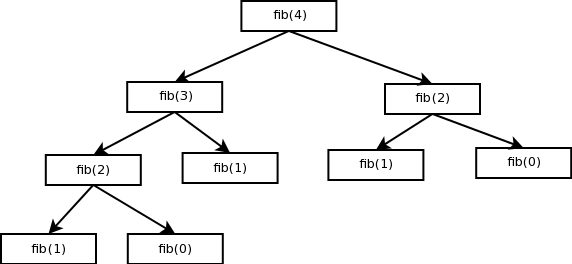
\includegraphics[height=0.6\textheight]{fibonacci_call_graph.png}}
\end{frame}

\begin{frame}[fragile]
\frametitle{Fibonacci - Without Memoization}


\begin{Verbatim}[commandchars=\\\{\}]
\PY{o}{>>}\PY{o}{>}\PY{+w}{ }\PY{n}{math\PYZus{}funcs}\PY{o}{.}\PY{n}{fibonacci}\PY{p}{(}\PY{l+m+mi}{4}\PY{p}{)}\PY{+w}{ }\PY{+w}{ }\PY{+w}{ }\PY{c}{\PYZsh{}}\PY{+w}{ }\PY{c}{9}\PY{+w}{ }\PY{c}{function}\PY{+w}{ }\PY{c}{calls}
\PY{n}{fibonacci}\PY{p}{(}\PY{l+m+mi}{4}\PY{p}{)}
\PY{n}{fibonacci}\PY{p}{(}\PY{l+m+mi}{3}\PY{p}{)}
\PY{n}{fibonacci}\PY{p}{(}\PY{l+m+mi}{2}\PY{p}{)}
\PY{n}{fibonacci}\PY{p}{(}\PY{l+m+mi}{1}\PY{p}{)}
\PY{n}{fibonacci}\PY{p}{(}\PY{l+m+mi}{0}\PY{p}{)}
\PY{n}{fibonacci}\PY{p}{(}\PY{l+m+mi}{1}\PY{p}{)}
\PY{n}{fibonacci}\PY{p}{(}\PY{l+m+mi}{2}\PY{p}{)}
\PY{n}{fibonacci}\PY{p}{(}\PY{l+m+mi}{1}\PY{p}{)}
\PY{n}{fibonacci}\PY{p}{(}\PY{l+m+mi}{0}\PY{p}{)}
\PY{l+m+mi}{3}
\end{Verbatim}

\end{frame}

\begin{frame}[fragile]
\frametitle{Fibonacci - With Memoization}


\begin{Verbatim}[commandchars=\\\{\}]
\PY{o}{>>}\PY{o}{>}\PY{+w}{ }\PY{n}{math\PYZus{}funcs}\PY{o}{.}\PY{n}{mfibonacci}\PY{p}{(}\PY{l+m+mi}{4}\PY{p}{)}\PY{+w}{ }\PY{+w}{ }\PY{c}{\PYZsh{}}\PY{+w}{ }\PY{c}{5}\PY{+w}{ }\PY{c}{function}\PY{+w}{ }\PY{c}{calls}
\PY{n}{fibonacci}\PY{p}{(}\PY{l+m+mi}{4}\PY{p}{)}
\PY{n}{fibonacci}\PY{p}{(}\PY{l+m+mi}{3}\PY{p}{)}
\PY{n}{fibonacci}\PY{p}{(}\PY{l+m+mi}{2}\PY{p}{)}
\PY{n}{fibonacci}\PY{p}{(}\PY{l+m+mi}{1}\PY{p}{)}
\PY{n}{fibonacci}\PY{p}{(}\PY{l+m+mi}{0}\PY{p}{)}
\PY{l+m+mi}{3}
\end{Verbatim}


\pause

\begin{Verbatim}[commandchars=\\\{\}]
\PY{o}{>>}\PY{o}{>}\PY{+w}{ }\PY{n}{math\PYZus{}funcs}\PY{o}{.}\PY{n}{mfibonacci}\PY{p}{(}\PY{l+m+mi}{4}\PY{p}{)}\PY{+w}{ }\PY{+w}{ }\PY{c}{\PYZsh{}}\PY{+w}{ }\PY{c}{No}\PY{+w}{ }\PY{c}{function}\PY{+w}{ }\PY{c}{calls}
\PY{l+m+mi}{3}\PY{+w}{ }\PY{+w}{ }\PY{+w}{ }\PY{+w}{ }\PY{+w}{ }\PY{+w}{ }\PY{+w}{ }\PY{+w}{ }\PY{+w}{ }\PY{+w}{ }\PY{+w}{ }\PY{+w}{ }\PY{+w}{ }\PY{+w}{ }\PY{+w}{ }\PY{+w}{ }\PY{+w}{ }\PY{+w}{ }\PY{+w}{ }\PY{+w}{ }\PY{+w}{ }\PY{+w}{ }\PY{+w}{ }\PY{+w}{ }\PY{+w}{ }\PY{+w}{ }\PY{+w}{ }\PY{+w}{ }\PY{+w}{ }\PY{c}{\PYZsh{}}\PY{+w}{ }\PY{c}{cache}\PY{+w}{ }\PY{c}{already}\PY{+w}{ }\PY{c}{has}\PY{+w}{ }\PY{c}{results}
\end{Verbatim}

\end{frame}

\begin{frame}[fragile]
\frametitle{References}

\begin{itemize}

\item \url{http://wiki.python.org/moin/PythonDecoratorLibrary\#Memoize}

\item Guide to: Learning Python Decorators by Matt Harrison
\url{http://www.amazon.com/Guide-Learning-Python-Decorators-ebook/dp/B006ZHJSIM/}
\end{itemize}
\end{frame}

\end{document}
